% compile with $ pdflatex project_plan
\documentclass{article}
\usepackage[margin=1in]{geometry}
\usepackage{fancyhdr}
\usepackage{graphicx}
\usepackage{vhistory}
\usepackage[parfill]{parskip}
\graphicspath{{../Images/}}

% Set fancy looking header/footer and move page number to the right
\pagestyle{fancy}
\fancyhead{}
\fancyfoot{}
\fancyfoot[R]{\thepage}

\title{}
\author{}
\date{}

\begin{document}

    \pagenumbering{gobble}
    \begin{titlepage}
    \begin{center}
        \vspace*{1cm}

        \Huge
        \textbf{User's Guide for Cloud Backup}

        \vspace{.5cm}
        \LARGE
        Captain CyBeard: Neil Before Us

        \vspace{1cm}

        \textbf{Ryan Breitenfeldt \textbar\ Noah Farris\\ Trevor Surface \textbar\ Kyle Thomas}

        \vspace{.2cm}
        \Large
        May 4, 2020

        \vspace{2cm}
        
\includegraphics[scale=1]{logo}

        \vfill

        Washington State University Tri-Cities\\
        CptS 423 Software Design Project 2

    \end{center}
\end{titlepage}



    \tableofcontents
    \newpage
    \listoffigures

    \newpage
    \begin{versionhistory}
        \vhEntry{2.0}{12.08.2019}{KT}{Added new gantt chart}
        \vhEntry{1.1}{11.12.2019}{KT}{Performed Edits}
        \vhEntry{1.0}{09.27.2019}{RB NF TS KT}{Completed Document}
        \vhEntry{0.5}{09.27.2019}{RB}{Filled in Estimate section}
        \vhEntry{0.4}{09.26.2019}{KT}{Filled in Approach section}
        \vhEntry{0.3}{09.24.2019}{RB NF TS KT}{Filled in scope and added diagram}
        \vhEntry{0.2}{09.19.2019}{KT}{Filled in Introduction Section}
        \vhEntry{0.1}{09.12.2019}{KT}{Document Creation}
    \end{versionhistory}
    \newpage

    \pagenumbering{arabic}

    \section{Introduction}
    This document is a project plan for developing a Django Web Application that allows Cypherpath users to enter
    a URL for online Virtual Machines and select which Virtual Machines will be downloaded onto Cypherpath's 
    servers. The purpose of the project plan is to provide a roadmap for CypherPath and the software development
    team of the development process and help keep track of the progress.

    Cypherpath is a company that provides a product called \textit{Resiliency Platform Tool} that stores virtual networks, machines, configurations and more
    enabling their customers to quickly recover from cyber attacks such as ransomware. Currently, customers need to manually download their virtual disk images from
    the various cloud platforms they are subscribed to (such as VMware or Amazon Web Services) and then upload them to Cypherpath's platform. This application will allow
    customers to have their virtual disk images transferred directly into the Resiliency Platform.

    Subsequent sections of this project plan will cover the scope of the project, the software engineering
    approach that will be used for the project and an estimate for how long the project will take broken by task
    in the form of a Gantt Chart.

    \section{Scope}
    The project is to develop a Python-Django web application that allows a user that is logged into the application to enter a URL that points to one of several
    possible cloud based VM platforms and be presented with the authentication for that platform. After the user enters their credentials for the VM platform 
    they will be presented with the virtual disk images they have on their account that are available to download. These virtual disk images are Cypherpath's customers
    virtualized appliances that are used for their business tasks.
    
    The application will present relevant information to the user such as the directory structure, names of the VM images, and a way to select which files and folders
    to download to their local machine.

    The first platform to focus on for interacting with will be VMware. Time permitting, other platforms such as Amazon Web Services (AWS), Citrix, Google Drive and Dropbox
    will be added. The application will have a modular design with both cloud platforms and authentication mechanisms so more can be added in the future.

    \begin{figure}[h]
    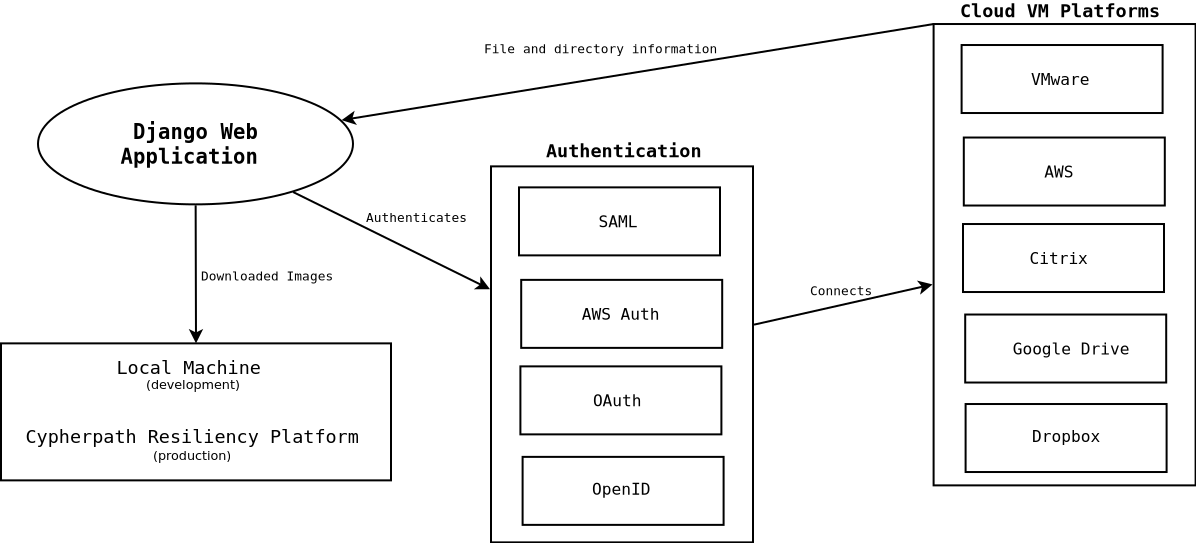
\includegraphics[scale=.4]{downloader_env}
        \caption{The application environment}
    \end{figure}

    \pagebreak
    \section{Approach}
    The software engineering approach that will be used for this project is the \textbf{Agile Scrum} approach.
    This iterative approach will ensure that the software development team will remain on track and that Cypherpath will receive the maximum amount of value
    for their time.

    The project will be implemented as a Python-Django web application, Python version 3+ and Django version 2+ will be used. The Python-Django framework provides the tools 
    and environment needed to develop and test a web application such as a lightweight web server and SQLite. For version control the software development team will be using git
    with a remote repository hosted on Github. Once the project is completed, Cypherpath will host the web application within their infrastructure.

    \section{Estimate}
    The project is estimated to take two academic semesters in order to complete collecting requirements, designing, implementation and testing. The estimated date
    to complete the project is Wednesday April 4th, 2020. The project is estimated to take 375 hours to complete.

    The following page will contain a breakdown of the tasks and estimated time to complete them for the project.

\end{document}
